\appendix
\chapter{WSDL}
\label{WSDL}

\section{Web Service Description Language}

\subsection{XML: el lenguaje de los WS's}

Si bien WSDL (Web Service Description Language) es en realidad el lenguaje de especificación utilizado para definir los WS's, esencialmente se trata de un documento XML que es utilizado para describir los mensajes SOAP y cómo estos mensajes son intercambiados.

\subsubsection*{Significado de XML}

XML es el estándar de Extensible Markup Language. XML es un metalenguaje que define la sintaxis utilizada para definir otros lenguajes de etiquetas estructurados.
Respecto a sus objetivos, estos son:

\begin{itemize}
	\item XML debe ser directamente utilizable sobre Internet.
	\item XML debe soportar una amplia variedad de aplicaciones.
	\item XML debe ser compatible con SGML.
	\item Debe ser fácil la escritura de programas que procesen documentos XML.
	\item El número de características opcionales en XML debe ser absolutamente mínimo, idealmente cero.
	\item Los documentos XML deben ser legibles por humanos y razonablemente claros.
	\item El diseño de XML debe ser preparado rápidamente.
	\item El diseño de XML debe ser formal y conciso.
	\item Los documentos XML deben ser fácilmente creables.
	\item La concisión en las marcas XML es de mínima importancia.
\end{itemize}


Por otra parte, se pueden enumerar sus principales características:
\begin{enumerate}[1.]
\item Es una arquitectura abierta y extensible. No se necesita versiones para que puedan funcionar en futuros navegadores. Los identificadores pueden crearse de manera simple y ser adaptados en el acto en internet/intranet por medio de un validador de documentos.
\item Mayor consistencia, homogeneidad y amplitud de los identificadores descriptivos del documento con XML (los RDF Resource Description FrameWork), en comparación a los atributos de la etiqueta del HTML. 
\item Integración de los datos de las fuentes más dispares. Se podrá hacer el intercambio de documentos entre las aplicaciones tanto en el propio PC como en una red local o extensa.
\item Datos compuestos de múltiples aplicaciones. La extensibilidad y flexibilidad de este lenguaje nos permitirá agrupar una variedad amplia de aplicaciones, desde páginas web hasta bases de datos.
\item Gestión y manipulación de los datos desde el propio cliente web. 
\item Los motores de búsqueda devolverán respuestas más adecuadas y precisas, ya que la codificación del contenido web en XML consigue que la estructura de la información resulte más accesible. 
\item Se desarrollarán de manera extensible las búsquedas personalizables y subjetivas para robots y agentes inteligentes. También conllevará que los clientes web puedan ser más autónomos para desarrollar tareas que actualmente se ejecutan en el servidor.
\item Se permitirá un comportamiento más estable y actualizable de las aplicaciones web, incluyendo enlaces bidireccionales y almacenados de forma externa (El famoso epígrafe "404 file not found" desaparecerá).
\item El concepto de "hipertexto" se desarrollará ampliamente (permitirá denominación independiente de la ubicación, enlaces bidireccionales, enlaces que pueden especificarse y gestionarse desde fuera del documento, hiperenlaces múltiples, enlaces agrupados, atributos para los enlaces, etc. Creado a través del Lenguaje de enlaces extensible (XLL).
\item Exportabilidad a otros formatos de publicación (papel, web, CD-ROM, etc.). El documento maestro de la edición electrónica podría ser un documento XML que se integraría en el formato deseado de manera directa.
\end{enumerate}

\subsubsection*{Estructura del XML}

El metalenguaje XML consta de cuatro especificaciones :
\begin{enumerate}[1.]
\item \textbf{DTD (Document Type Definition)} Definición del tipo de documento. Es, en general, un archivo que encierra una definición formal de un tipo de documento y, a la vez, especifica la estructura lógica de cada documento. Define tanto los elementos de una página como sus atributos. El DTD del XML es opcional. 

\item \textbf{XSL (eXtensible Stylesheet Language)} Define o implementa el lenguaje de estilo de los documentos escritos para XML.. Permite modificar el aspecto de un documento.
Se puede lograr múltiple columnas, texto girado, orden de visualización de los datos de una tabla, múltiples tipos de letra con amplia variedad en los tamaños. Este estándar está basado en el lenguaje de semántica y especificación de estilo de documento (DSSSL, Document Style Semantics  and Specification Language, ISO/IEC 10179).

\item \textbf{XLL (eXtensible Linking Language)} Define el modo de enlace entre diferentes enlaces. Se considera que es un subconjunto de HyTime (Hipermedia/Timed-based structuring Language ó Lenguaje de estructuración hipermedia/basado en el tiempo, ISO 10744) y sigue algunas especificaciones del TEI (Text Encoding Initiative o Iniciativa de codificación de texto). \\
Este lenguaje de enlaces extensible tiene dos importantes componentes: Xlink y el Xpointer. Va más allá de los enlaces simples que sólo soporta el HTML. Se podrá implementar con enlaces extendidos. Jon Bosak establece los siguientes mecanismos hipertextuales que soportará esta especificación:\\
\begin{itemize}
	\item Denominación independiente de la ubicación.
	\item Enlaces que pueden especificarse y gestionarse desde fuera del documento a los que se apliquen.
	\item Hiperenlaces múltiples.
	\item Enlaces agrupados.
	\item Transclusión (el documento destino al que apunta el enlace aparece como parte integrante del documento rigen del enlace).
	\item Se pueden aplicar atributos a los enlaces.
\end{itemize}


\item \textbf{XUA (XML User Agent)} Estandarización de navegadores XML.\\
Todavía está en proceso de creación de borradores de trabajo. Se aplicará a los navegadores para que compartan todas las especificaciones XML
\end{enumerate}

\subsection{WSDL y la documentación de WS's}

El lenguaje de descripción de WS's (WSDL, Web Service Description Language) es un dialecto basado en XML sobre el esquema que describe un WS. Un documento WSDL proporciona la información necesaria al cliente para interaccionar con el WS. \\
Los documentos WSDL definen los servicios como colecciones de puntos finales de red o puertos. En WSDL, la definición abstracta de puntos finales y de mensajes se separa de la instalación concreta de red o de los enlaces del formato de datos. Esto permite la reutilización de definiciones abstractas: mensajes, que son descripciones abstractas de los datos que se están intercambiando y tipos de puertos, que son colecciones abstractas de operaciones. Las especificaciones concretas del protocolo y del formato de datos para un tipo de puerto determinado constituyen un enlace reutilizable. Un puerto se define por la asociación de una dirección de red y un enlace reutilizable; una colección de puertos define un servicio. Por esta razón, un documento WSDL utiliza los siguientes elementos en la definición de servicios de red: 

\begin{itemize}
	\item Types: contenedor de definiciones del tipo de datos que utiliza algún sistema de tipos.
	\item Message: definición abstracta y escrita de los datos que se están comunicando.
	\item Operation: descripción abstracta de una acción admitida por el servicio.
	\item Port Type: conjunto abstracto de operaciones admitidas por uno o más puntos finales.
	\item Binding: especificación del protocolo y del formato de datos para un tipo de puerto determinado.
	\item Port: punto final único que se define como la combinación de un enlace y una dirección de red.
	\item Service: colección de puntos finales relacionados.
\end{itemize}

\subsection{WSDL y la descripción de los WS's}

WSDL separa la descripción de un servicio en dos partes. Una de ellas es la interfaz abstracta, la cual describe las operaciones soportadas por el servicio, los parámetros de la operación y los tipos de datos abstractos. La otra parte es la implementación concreta, la cual liga la interfaz abstracta a una dirección de red, protocolo y estructuras de datos concretas. WSDL provee toda esta información a través de elementos XML. \\
Además, la descripción de un WS tiene dos componentes principales: sus características funcionales y no funcionales. La descripción funcional detalla las características operacionales que definen el comportamiento general de un WS. La descripción no funcional se concentra en sus atributos de calidad (Quality of Service - QoS), forzando al solicitante del servicio a especificar, los atributos de calidad que pueden influir en la elección de un WS ofrecido por un proveedor.

\subsection{Estructura de un documento WSDL}

En la primera versión de este lenguaje, WSDL 1.1, el documento que describe un WS está compuesto por un elemento raíz llamado definitions, que a su vez está compuesto por los siguientes elementos:

\begin{itemize}
	\item \textbf{types:} provee la definición de los tipos de datos utilizados para describir los mensajes a intercambiar.
	\item \textbf{message:} representa una definición abstracta de los datos a ser transmitidos entre el servidor y el cliente.
	\item \textbf{portType:} define un conjunto de operaciones abstractas. Cada operación se refiere a un mensaje de entrada y mensajes de salida.
	\item \textbf{binding:} define un protocolo concreto y las especificaciones de formato de datos para las operaciones y los mensajes definidos en un portType particular.
	\item \textbf{port:} el cual especifica una dirección de enlace, definiendo un punto final de comunicación.
	\item \textbf{service:} se usa para agrupar un conjunto de puertos relacionados.
\end{itemize}

La nueva versión de este lenguaje, WSDL 2.0 \cite{WSDL2.0-0}, hereda la mayoría de los principios arquitecturales de WSDL 1.1 e incorpora, los conceptos de interface abstracta, protocolo de enlace (binding), y puntos finales de servicios (service endpoints). Algunos de los cambios incorporados en WSDL 2.0 son:\\
Agrega más semántica al lenguaje de descripción;\\
Remueve el elemento message: este se especifica dentro del elemento types, usando XML Schema Type System;\\
No soporta la sobrecarga de operadores;\\

Renombra el elemento portTypes a interfaces: La herencia de interfaces se consigue el atributo extends en el elemento interface;\\
Renombra los ports a endpoints;\\
Incorpora patrones de mensajes abstractos.\\

En esta versión los elementos principales que componen el documento que describe el WS, los cuales están contenidos en el elemento description, son: \\
\begin{itemize}
	\item \textbf{types:} provee la definición de los tipos de datos utilizados para describir los mensajes a intercambiar.
	\item \textbf{interface:} describe la secuencia de mensajes que el servicio envía o recibe.
	\item \textbf{binding:} define un protocolo concreto y las especificaciones de formato de datos para las operaciones y los mensajes definidos en un portType particular.
	\item \textbf{service:} se usa para agrupar un conjunto de puertos relacionados.
\end{itemize}

La sección abstracta contiene los elementos types e interface (message y operations), mientras que la sección concreta contiene los elementos binding y service.

\begin{figure}[!h] 
	\begin{center}
		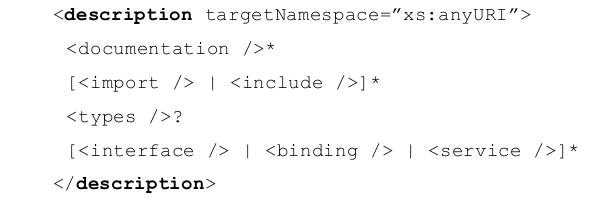
\includegraphics [scale=0.70]{imagenes/descripcion_ws.png}
	\end{center}
	\caption{Descripción de un WS}
	\label{fig:Descripción de un WS}
\end{figure} 

\subsubsection*{El Elemento Types}

El elemento types incluye la definición de los tipos de datos que son relevantes para el intercambio de mensajes y que se necesitarán posteriormente para la definición. Ellos son los parámetros de entrada y salida respectivamente.(ver figura \ref{fig:Elemento Types de un WS})

\begin{figure}[!h] 
	\begin{center}
		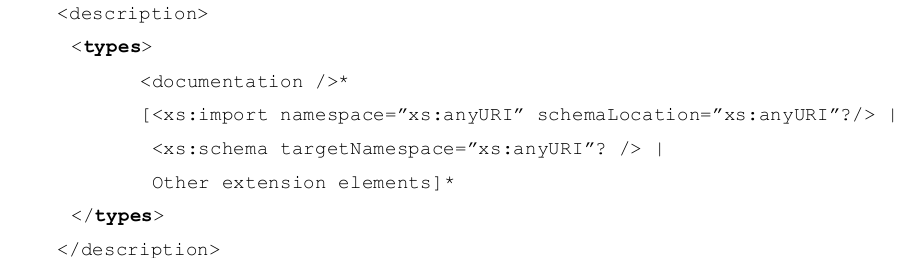
\includegraphics [scale=0.43]{imagenes/elemento_types.png}
	\end{center}
	\caption{Elemento Types de un WS}
	\label{fig:Elemento Types de un WS}
\end{figure} 

\subsubsection*{El Elemento Interface}

El elemento interface describe la secuencia de mensajes que el servicio envía o recibe. Para ello agrupa los mensajes en operaciones. Una operación es una secuencia de mensajes de entrada y salida, y una interface es un conjunto de operaciones.(ver figura \ref{fig:Elemento Interface de un WS})\\
El conjunto de operaciones disponibles en un interface incluye todas las operaciones definidas por las interfaces que ella extiende, directa o indirectamente, más las operaciones que ella define directamente. Las propiedades de una interface son:\\

\begin{itemize}
	\item Nombre (name).
	\item Interfaces que extiende (extends).
	\item Componentes de falla (fault): describe las fallas que pueden ocurrir durante la \item invocación de una operación de la interface.
	\item Operaciones (operation): describe una operación que ocurre dentro de la interface que la soporta. Una operación es una interacción con el servicio, que consiste de un conjunto de mensajes intercambiados entre el servicio y las otras partes involucradas en la interacción.
\end{itemize}

\begin{figure}[!h] 
	\begin{center}
		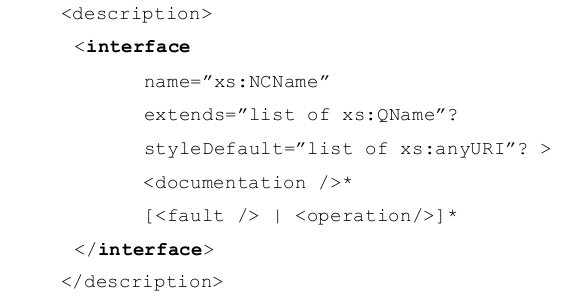
\includegraphics [scale=0.70]{imagenes/elemento_interface.png}
	\end{center}
	\caption{Elemento Interface de un WS}
	\label{fig:Elemento Interface de un WS}
\end{figure} 

\subsubsection*{El Elemento Binding}

El elemento Binding define los detalles de implementación concretos, que serán necesarios para acceder al servicio.(ver figura \ref{fig:Elemento Binding de un WS})

\begin{figure}[!h] 
\begin{center}
	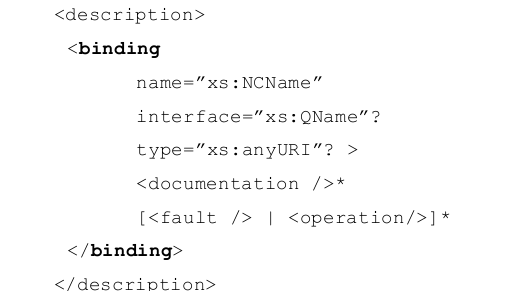
\includegraphics [scale=0.70]{imagenes/elemento_binding.png}
\end{center}
\caption{Elemento Binding de un WS}
\label{fig:Elemento Binding de un WS}
\end{figure} 

El binding debe especificar la interface a la que se aplica y definir bindings para todas las fallas definidas en la interface, que son referenciadas en las operaciones.
Las propiedades de este componente son:\\
\begin{itemize}
	\item nombre (name).
	\item interface (interface), para la cual se especifica el componente binding.
	\item tipo (type), que indica los detalles de binding concretos.
	\item falla (binding faults): describe un binding concreto para una falla particular descripta dentro de la interface.
	\item operaciones (binding operations): define el formato de mensaje concreto y el protocolo de interacción asociados con una operación de interface particular.
\end{itemize}

\subsubsection*{El Elemento Service}

El elemento Service asocia un binding con el URL donde está realmente el servicio a través de un endpoint. Los endpoints son lugares alternativos que proveen el servicio. (ver figura \ref{fig:Elemento Service de un WS})

\begin{figure}[!h] 
	\begin{center}
		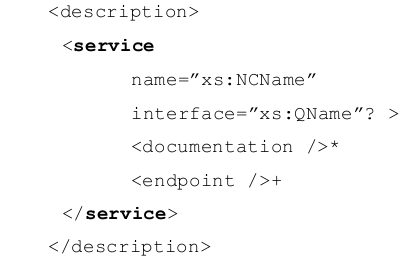
\includegraphics [scale=0.70]{imagenes/elemento_service.png}
	\end{center}
	\caption{Elemento Service de un WS}
	\label{fig:Elemento Service de un WS}
\end{figure} 

Las propiedades de este componente son:
\begin{itemize}
	\item nombre (name).
	\item interface (interface), la interface que el servicio instancia.
	\item punto final (endpoint): define las particularidades de un punto final específico en el cual el servicio está disponible.
\end{itemize}

\subsubsection*{Elemento message}

El elemento Message proporciona una abstracción común para el paso de mensajes entre el cliente y el servidor. Como puede utilizar múltiples formatos de definición de esquema en documento WSDL es necesario de disponer de un mecanismo común de identificar los mensajes. El elemento Message proporciona este nivel común de abstracción al que se hará referencia en otras partes del documento WSDL. Cada mensaje contiene uno o más elementos "Part" que describen las piezas del contenido del mensaje.

\subsubsection*{Elemento portType}

El elemento portType contiene un conjunto de operaciones abstractas que representan los tipos de correspondencia que pueden producirse entre el cliente y el servidor.
WSDL define cuatro tipos de operaciones:

\begin{itemize}
	\item Request-response (petición-respuesta). Comunicación del tipo RPC en la que el cliente realiza una petición y el servidor envía la correspondiente respuesta.
	\item One-way (un-sentido). Comunicación del estilo documento en la que el cliente envía un mensaje pero no recibe una respuesta del servidor indicando el resultado del mensaje procesado.
	\item Solicit-response (solicitud-respuesta). La contraria a la operación petición-respuesta. El servidor envía una petición y el cliente le envía de vuelta una respuesta.
	\item Notification (Notificación). La contraria a la operación un-sentido el servidor envía una comunicación del estilo documento al cliente.
\end{itemize}

\subsubsection{Elementos de Extensibilidad}

Los elementos de extensibilidad se utilizan para representar determinadas tecnologías.

